\documentclass[11pt,a4paper]{article}

\usepackage[margin=22mm,headheight=14pt]{geometry}

\usepackage{longtable,booktabs,array,hyperref,xcolor,tikz,fancyhdr}

\usepackage{fontspec,xeCJK}

\setmainfont[Ligatures=TeXOff]{Times New Roman}

\setsansfont[Ligatures=TeXOff]{Times New Roman}

\setmonofont[Ligatures=TeXOff,WordSpace={1,1,1}]{Times New Roman}

\setCJKmainfont{Noto Serif CJK SC}

\setCJKsansfont{Noto Serif CJK SC}

\setCJKmonofont{Noto Serif CJK SC}

\XeTeXgenerateactualtext=1

\definecolor{vulcan}{HTML}{BB3E23}

\pgfdeclarelayer{connections}\pgfdeclarelayer{edge labels}\pgfsetlayers{connections,main,edge labels}

\hypersetup{hidelinks}

\newcolumntype{L}[1]{>{\raggedright\arraybackslash}p{#1}}

\setlength{\emergencystretch}{5em}\tolerance=2000\hbadness=10000

\setlength{\parindent}{0pt}\setlength{\parskip}{5pt}

\pagestyle{fancy}\fancyhf{}\fancyhead[L]{\small\sffamily VULCAN}

\fancyhead[R]{\small Product design and verification}\fancyfoot[C]{\thepage}

\begin{document}

{\sffamily\huge\raggedright\textbf{Anvil-E2: Programmable Vision and Text Embedding RTL}\par}

{\large Technical Design and Verification Report}\par

15 October 2026 (\allowbreak{}UTC+\allowbreak{}8)\allowbreak{}\par\textcolor{vulcan}{\rule{\textwidth}{0.5pt}}

\begin{abstract}

Anvil-E2 is a modular,\allowbreak{} synthesizable SystemVerilog inference datapath implementing the supplied EmbeddingGemma-2 vision-and-text architecture. It integrates patch embedding,\allowbreak{} a reusable vision transformer,\allowbreak{} spatial pooling and projection,\allowbreak{} multimodal framing,\allowbreak{} per-layer input injection,\allowbreak{} a hybrid text transformer,\allowbreak{} masked mean pooling and prefix-selectable L2 normalization.


The implementation combines signed Q8.24 external words with Q8.40 stage-local arithmetic. Independent public-pin verification passed 36 mandatory configuration,\allowbreak{} seed,\allowbreak{} mode and output-length combinations. Maximum normalized-component error was 2.830035e-5 and maximum nonzero-vector L2-norm error was 4.471436e-8,\allowbreak{} both below 0.002. Five executable defect mutations were rejected,\allowbreak{} and generic synthesis of two scaled configurations found zero latches. These results establish synthetic-workload RTL behavior,\allowbreak{} not pretrained-model quality or physical chip performance.


\end{abstract}

\section{Architecture and design rationale}

Anvil-E2 trades parallel throughput for bounded local storage and reusable arithmetic. A registered controller sequences seven literal processing stages through a single-outstanding memory bridge. One vision-layer engine serves all configured vision layers,\allowbreak{} and one text-layer engine serves all text layers. Intermediate tensors reside in external scratch; local banks hold bounded vectors rather than complete frames or model tables. Specialized frontend,\allowbreak{} layer and output instances retain their required operators without elaborating irrelevant helpers. Registered clock ownership isolates inactive stages and selected arithmetic helpers; the controller and memory bridge remain clocked. Blocks are arranged row-major for a three-column diagram. Links identify control relationships or scratch-mediated tensor dependencies,\allowbreak{} not direct streaming connections between processing stages.

\begin{center}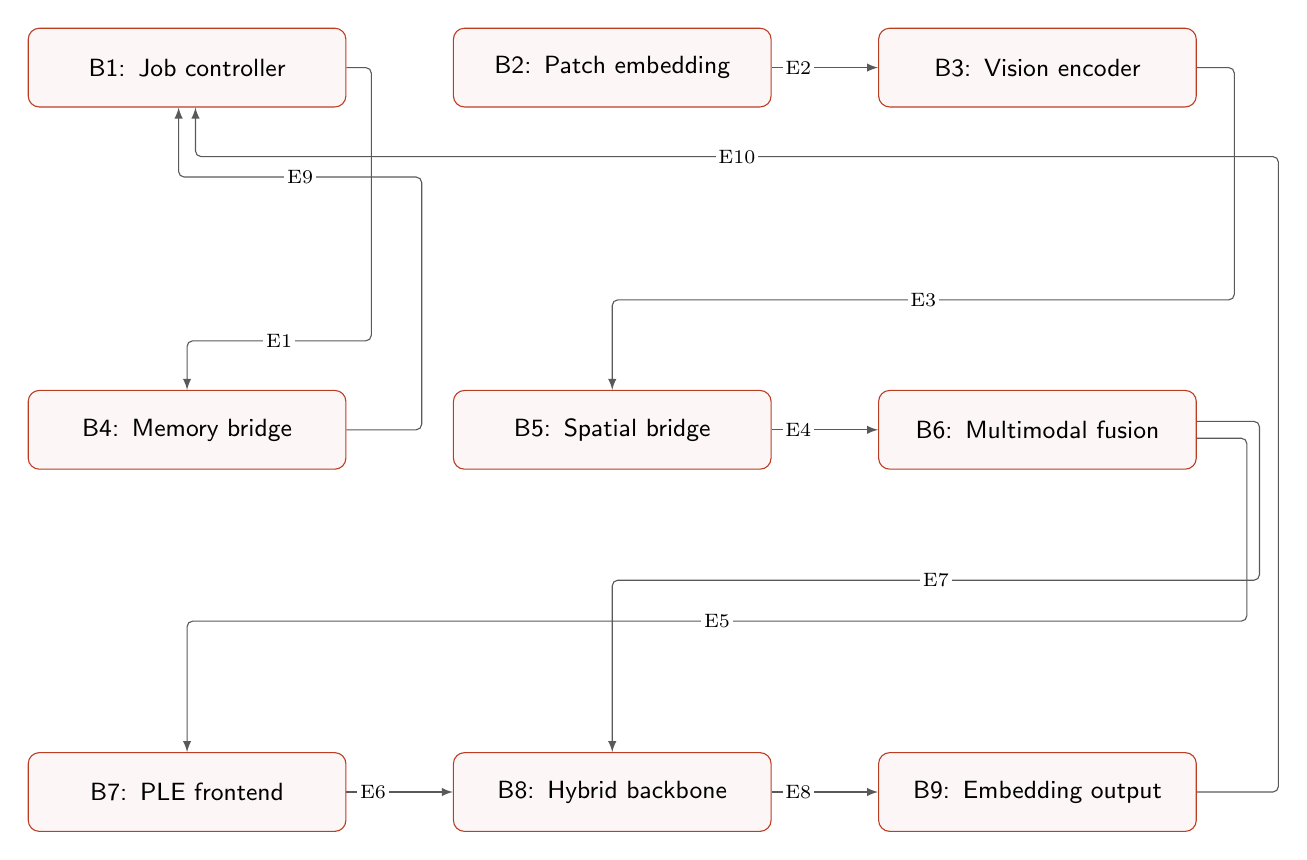
\begin{tikzpicture}[every node/.style={font=\small\sffamily},>=latex]

\node[draw=vulcan,rounded corners,fill=vulcan!4,text width=3.8cm,minimum height=1cm,align=center] (b0) at (0.0,0.0) {B1: Job controller};

\node[draw=vulcan,rounded corners,fill=vulcan!4,text width=3.8cm,minimum height=1cm,align=center] (b1) at (5.4,0.0) {B2: Patch embedding};

\node[draw=vulcan,rounded corners,fill=vulcan!4,text width=3.8cm,minimum height=1cm,align=center] (b2) at (10.8,0.0) {B3: Vision encoder};

\node[draw=vulcan,rounded corners,fill=vulcan!4,text width=3.8cm,minimum height=1cm,align=center] (b3) at (0.0,-4.6) {B4: Memory bridge};

\node[draw=vulcan,rounded corners,fill=vulcan!4,text width=3.8cm,minimum height=1cm,align=center] (b4) at (5.4,-4.6) {B5: Spatial bridge};

\node[draw=vulcan,rounded corners,fill=vulcan!4,text width=3.8cm,minimum height=1cm,align=center] (b5) at (10.8,-4.6) {B6: Multimodal fusion};

\node[draw=vulcan,rounded corners,fill=vulcan!4,text width=3.8cm,minimum height=1cm,align=center] (b6) at (0.0,-9.2) {B7: PLE frontend};

\node[draw=vulcan,rounded corners,fill=vulcan!4,text width=3.8cm,minimum height=1cm,align=center] (b7) at (5.4,-9.2) {B8: Hybrid backbone};

\node[draw=vulcan,rounded corners,fill=vulcan!4,text width=3.8cm,minimum height=1cm,align=center] (b8) at (10.8,-9.2) {B9: Embedding output};

\begin{pgfonlayer}{connections}

\draw[->,black!65,rounded corners=2pt] ([yshift=0.000cm]b0.east) -- (2.340,0.000) -- (2.340,-3.470) -- coordinate[midway] (e0) (0.000,-3.470) -- ([xshift=0.000cm]b3.north);

\draw[->,black!65] ([yshift=0.000cm]b1.east) -- coordinate[pos=0.25] (e1) ([yshift=0.000cm]b2.west);

\draw[->,black!65,rounded corners=2pt] ([yshift=0.000cm]b2.east) -- (13.300,0.000) -- (13.300,-2.950) -- coordinate[midway] (e2) (5.400,-2.950) -- ([xshift=0.000cm]b4.north);

\draw[->,black!65] ([yshift=0.000cm]b4.east) -- coordinate[pos=0.25] (e3) ([yshift=0.000cm]b5.west);

\draw[->,black!65,rounded corners=2pt] ([yshift=-0.107cm]b5.east) -- (13.460,-4.707) -- (13.460,-7.030) -- coordinate[midway] (e4) (0.000,-7.030) -- ([xshift=0.000cm]b6.north);

\draw[->,black!65] ([yshift=0.000cm]b6.east) -- coordinate[pos=0.25] (e5) ([yshift=0.000cm]b7.west);

\draw[->,black!65,rounded corners=2pt] ([yshift=0.107cm]b5.east) -- (13.620,-4.493) -- (13.620,-6.510) -- coordinate[midway] (e6) (5.400,-6.510) -- ([xshift=0.000cm]b7.north);

\draw[->,black!65] ([yshift=0.000cm]b7.east) -- coordinate[pos=0.25] (e7) ([yshift=0.000cm]b8.west);

\draw[->,black!65,rounded corners=2pt] ([yshift=0.000cm]b3.east) -- (2.980,-4.600) -- (2.980,-1.390) -- coordinate[midway] (e8) (-0.107,-1.390) -- ([xshift=-0.107cm]b0.south);

\draw[->,black!65,rounded corners=2pt] ([yshift=0.000cm]b8.east) -- (13.860,-9.200) -- (13.860,-1.130) -- coordinate[midway] (e9) (0.107,-1.130) -- ([xshift=0.107cm]b0.south);

\end{pgfonlayer}

\begin{pgfonlayer}{edge labels}

\node[fill=white,inner sep=1pt,font=\scriptsize] at (e0) {E1};

\node[fill=white,inner sep=1pt,font=\scriptsize] at (e1) {E2};

\node[fill=white,inner sep=1pt,font=\scriptsize] at (e2) {E3};

\node[fill=white,inner sep=1pt,font=\scriptsize] at (e3) {E4};

\node[fill=white,inner sep=1pt,font=\scriptsize] at (e4) {E5};

\node[fill=white,inner sep=1pt,font=\scriptsize] at (e5) {E6};

\node[fill=white,inner sep=1pt,font=\scriptsize] at (e6) {E7};

\node[fill=white,inner sep=1pt,font=\scriptsize] at (e7) {E8};

\node[fill=white,inner sep=1pt,font=\scriptsize] at (e8) {E9};

\node[fill=white,inner sep=1pt,font=\scriptsize] at (e9) {E10};

\end{pgfonlayer}

\end{tikzpicture}\end{center}

{\small Functional block map, not a gate-level netlist. Edge identifiers match the directed relationships below. Crossings do not denote junctions; separate attachment points preserve arrow directions.}

{\small\begin{longtable}{@{}L{0.24\textwidth}L{0.7\textwidth}@{}}\toprule

\textbf{Block} & \textbf{Responsibility}\\\midrule\endhead

B1: Job controller & anvil\_\allowbreak{}e2\_\allowbreak{}top captures descriptors,\allowbreak{} validates geometry and extents,\allowbreak{} registers stage ownership,\allowbreak{} iterates layers and holds completion.\\[3pt]

B2: Patch embedding & anvil\_\allowbreak{}e2\_\allowbreak{}vision\_\allowbreak{}patch\_\allowbreak{}embed reads RGB patches,\allowbreak{} performs dense projection and adds separate row and column position factors.\\[3pt]

B3: Vision encoder & anvil\_\allowbreak{}e2\_\allowbreak{}vision\_\allowbreak{}encoder\_\allowbreak{}layer executes reusable bidirectional attention and gated-feedforward layers with axial rotary encoding.\\[3pt]

B4: Memory bridge & anvil\_\allowbreak{}e2\_\allowbreak{}memory converts selected-stage commands into stable external requests and registered responses,\allowbreak{} including write acknowledgments.\\[3pt]

B5: Spatial bridge & anvil\_\allowbreak{}e2\_\allowbreak{}vision\_\allowbreak{}pool\_\allowbreak{}proj averages spatial-window participants and projects vision vectors into text hidden space.\\[3pt]

B6: Multimodal fusion & anvil\_\allowbreak{}e2\_\allowbreak{}multimodal\_\allowbreak{}fusion constructs framed IDs,\allowbreak{} positions,\allowbreak{} masks and initial hidden vectors for image and text modes.\\[3pt]

B7: PLE frontend & anvil\_\allowbreak{}e2\_\allowbreak{}text\_\allowbreak{}frontend\_\allowbreak{}ple computes and materializes each token's per-layer input vectors from its initial fused hidden state.\\[3pt]

B8: Hybrid backbone & anvil\_\allowbreak{}e2\_\allowbreak{}hybrid\_\allowbreak{}layer performs sliding or full grouped attention,\allowbreak{} gated MLP,\allowbreak{} cached per-layer input injection and scalar multiplication.\\[3pt]

B9: Embedding output & anvil\_\allowbreak{}e2\_\allowbreak{}pool\_\allowbreak{}norm performs final language normalization,\allowbreak{} embedding projection,\allowbreak{} masked mean,\allowbreak{} prefix selection and L2 normalization.\\[3pt]

\bottomrule\end{longtable}}

{\small\begin{longtable}{@{}L{0.24\textwidth}L{0.7\textwidth}@{}}\toprule

\textbf{Directed relationship} & \textbf{Meaning}\\\midrule\endhead

E1: B1 to B4 & Selected-owner command routing\\[3pt]

E2: B2 to B3 & Projected patches through scratch\\[3pt]

E3: B3 to B5 & Final vision tensor through scratch\\[3pt]

E4: B5 to B6 & Projected soft tokens through scratch\\[3pt]

E5: B6 to B7 & Initial fused hidden tensor\\[3pt]

E6: B7 to B8 & Materialized per-layer input cache\\[3pt]

E7: B6 to B8 & Hidden state and fused metadata\\[3pt]

E8: B8 to B9 & Final hidden tensor and pooling masks\\[3pt]

E9: B4 to B1 & Bridge readiness and response ownership\\[3pt]

E10: B9 to B1 & Held stage completion and error\\[3pt]

\bottomrule\end{longtable}}

\section{Interfaces and configuration}

{\small\begin{longtable}{@{}L{0.2\textwidth}L{0.12\textwidth}L{0.1\textwidth}L{0.48\textwidth}@{}}\toprule

\textbf{Signal /\allowbreak{} group} & \textbf{Direction} & \textbf{Width} & \textbf{Contract}\\\midrule\endhead

clk,\allowbreak{} rst\_\allowbreak{}n & Input & 1 bit each & Rising-edge operation with asynchronous active-low reset. Asserted reset forces every public output to zero and cancels the active job and transaction.\\[3pt]

job\_\allowbreak{}valid /\allowbreak{} job\_\allowbreak{}ready & Input /\allowbreak{} output & 1 bit each & Captures the complete descriptor only when both signals are asserted at a rising edge. Only one job is outstanding.\\[3pt]

job\_\allowbreak{}mode,\allowbreak{} job\_\allowbreak{}tokens,\allowbreak{} job\_\allowbreak{}patch\_\allowbreak{}rows,\allowbreak{} job\_\allowbreak{}patch\_\allowbreak{}cols,\allowbreak{} job\_\allowbreak{}output\_\allowbreak{}dim & Input & 2,\allowbreak{} 32,\allowbreak{} 32,\allowbreak{} 32 and 16 bits & Modes 0,\allowbreak{} 1 and 2 select text-only,\allowbreak{} vision-only and joint execution; mode 3 is invalid. Vision-only requires zero supplied text tokens; joint requires a positive count.\\[3pt]

weights\_\allowbreak{}base,\allowbreak{} vision\_\allowbreak{}weights\_\allowbreak{}base,\allowbreak{} image\_\allowbreak{}base,\allowbreak{} tokens\_\allowbreak{}base,\allowbreak{} positions\_\allowbreak{}base,\allowbreak{} mask\_\allowbreak{}base,\allowbreak{} scratch\_\allowbreak{}base & Input & 64 bits each & Aligned byte addresses for weights,\allowbreak{} operands and scratch. Active host regions must be nonoverlapping and remain valid throughout execution.\\[3pt]

mem\_\allowbreak{}req\_\allowbreak{}valid,\allowbreak{} mem\_\allowbreak{}req\_\allowbreak{}write,\allowbreak{} mem\_\allowbreak{}req\_\allowbreak{}addr,\allowbreak{} mem\_\allowbreak{}req\_\allowbreak{}wdata /\allowbreak{} mem\_\allowbreak{}req\_\allowbreak{}ready & Output /\allowbreak{} input & 1,\allowbreak{} 1,\allowbreak{} 64,\allowbreak{} 32 /\allowbreak{} 1 bits & Little-endian,\allowbreak{} byte-addressed 32-bit memory requests. Payload remains stable while stalled. At most one accepted request awaits a response.\\[3pt]

mem\_\allowbreak{}rsp\_\allowbreak{}valid,\allowbreak{} mem\_\allowbreak{}rsp\_\allowbreak{}rdata,\allowbreak{} mem\_\allowbreak{}rsp\_\allowbreak{}error /\allowbreak{} mem\_\allowbreak{}rsp\_\allowbreak{}ready & Input /\allowbreak{} output & 1,\allowbreak{} 32,\allowbreak{} 1 /\allowbreak{} 1 bits & Exactly one response is required for each accepted read or write. A response cannot retire on the edge that accepts its request.\\[3pt]

emb\_\allowbreak{}valid,\allowbreak{} emb\_\allowbreak{}data,\allowbreak{} emb\_\allowbreak{}index,\allowbreak{} emb\_\allowbreak{}last /\allowbreak{} emb\_\allowbreak{}ready & Output /\allowbreak{} input & 1,\allowbreak{} signed 32,\allowbreak{} 16,\allowbreak{} 1 /\allowbreak{} 1 bits & Ordered Q8.24 embedding beats with zero-based indices. Data,\allowbreak{} index and last remain stable under backpressure. Output begins only after complete normalization.\\[3pt]

done\_\allowbreak{}valid,\allowbreak{} done\_\allowbreak{}error,\allowbreak{} busy /\allowbreak{} done\_\allowbreak{}ready & Output /\allowbreak{} input & 1,\allowbreak{} 4,\allowbreak{} 1 /\allowbreak{} 1 bits & Held completion and status. Final embedding acceptance precedes a separate completion phase. A new descriptor cannot be accepted on the completion-retirement edge.\\[3pt]

\bottomrule\end{longtable}}

{\small\begin{longtable}{@{}L{0.23\textwidth}L{0.12\textwidth}L{0.57\textwidth}@{}}\toprule

\textbf{Parameter} & \textbf{Default} & \textbf{Meaning /\allowbreak{} supported values}\\\midrule\endhead

VISION\_\allowbreak{}LAYERS,\allowbreak{} VISION\_\allowbreak{}HIDDEN,\allowbreak{} VISION\_\allowbreak{}FFN & 16,\allowbreak{} 768,\allowbreak{} 3072 & Positive and at most 65535; overrides change actual computation and bounded storage.\\[3pt]

VISION\_\allowbreak{}HEADS,\allowbreak{} VISION\_\allowbreak{}HEAD\_\allowbreak{}DIM & 12,\allowbreak{} 64 & Positive; VISION\_\allowbreak{}HIDDEN equals their product. Head dimension is divisible by four for row and column rotary partitions.\\[3pt]

PATCH\_\allowbreak{}SIZE,\allowbreak{} POOL\_\allowbreak{}KERNEL,\allowbreak{} VISION\_\allowbreak{}SOFT\_\allowbreak{}TOKENS & 16,\allowbreak{} 3,\allowbreak{} 280 & Positive; 3*\allowbreak{}PATCH\_\allowbreak{}SIZE*\allowbreak{}PATCH\_\allowbreak{}SIZE fits 65535. The ceiling-divided spatial-window count must equal VISION\_\allowbreak{}SOFT\_\allowbreak{}TOKENS.\\[3pt]

TEXT\_\allowbreak{}LAYERS,\allowbreak{} TEXT\_\allowbreak{}HIDDEN,\allowbreak{} PLE\_\allowbreak{}DIM,\allowbreak{} TEXT\_\allowbreak{}FFN & 24,\allowbreak{} 512,\allowbreak{} 512,\allowbreak{} 2048 & Positive and at most 65535. Singleton hidden,\allowbreak{} per-layer input and feedforward widths are supported.\\[3pt]

EMBED\_\allowbreak{}DIM & 768 & At least six,\allowbreak{} divisible by six and at most 65535. Allowed output lengths are B,\allowbreak{} 2B/\allowbreak{}3,\allowbreak{} B/\allowbreak{}3 and B/\allowbreak{}6.\\[3pt]

VOCAB\_\allowbreak{}SIZE,\allowbreak{} POSITION\_\allowbreak{}EMBEDDING\_\allowbreak{}SIZE & 262144,\allowbreak{} 10240 & Positive. Image jobs require vocabulary coverage through special ID 258882; patch-grid dimensions cannot exceed the position-table extent.\\[3pt]

TEXT\_\allowbreak{}Q\_\allowbreak{}HEADS,\allowbreak{} LOCAL\_\allowbreak{}KV\_\allowbreak{}HEADS,\allowbreak{} FULL\_\allowbreak{}KV\_\allowbreak{}HEADS & 4,\allowbreak{} 2,\allowbreak{} 1 & Positive; each KV count divides the query-head count. Contiguous query-head groups share KV heads.\\[3pt]

LOCAL\_\allowbreak{}HEAD\_\allowbreak{}DIM,\allowbreak{} FULL\_\allowbreak{}HEAD\_\allowbreak{}DIM & 256,\allowbreak{} 512 & Positive even dimensions; each query-head-count product fits 65535.\\[3pt]

SLIDING\_\allowbreak{}WINDOW,\allowbreak{} MAX\_\allowbreak{}SEQ\_\allowbreak{}LEN & 512,\allowbreak{} 262144 & Positive. Sequence and patch counts fit unsigned 32-bit counters; fused sequence length and positions obey MAX\_\allowbreak{}SEQ\_\allowbreak{}LEN.\\[3pt]

\bottomrule\end{longtable}}

\section{Behavior and corner cases}

\subsection{Vision processing and fusion}

The input image is externally preprocessed RGB CHW,\allowbreak{} without additional standardization. Patch flattening orders channel,\allowbreak{} row and column. Dense input projection is followed by separate factors from the two-axis position table. Each vision layer applies offset-scale RMS normalization,\allowbreak{} Q/\allowbreak{}K/\allowbreak{}V projection,\allowbreak{} per-head Q/\allowbreak{}K RMS,\allowbreak{} axial RoPE with theta 100,\allowbreak{} bidirectional softmax attention,\allowbreak{} output projection and normalized residual/\allowbreak{}feedforward operations. Spatial pooling uses nonoverlapping windows and averages actual participants in partial edge windows. Image sequences contain boi 255999,\allowbreak{} exactly S image slots tagged 258880,\allowbreak{} eoi 258882,\allowbreak{} then supplied text. Image vectors come from the dense bridge,\allowbreak{} not the image-token embedding row. Frame and text embeddings receive sqrt(\allowbreak{}TEXT\_\allowbreak{}HIDDEN)\allowbreak{} scaling; image vectors do not. Generated masks are one,\allowbreak{} and appended text positions shift by S+\allowbreak{}2.

\subsection{Hybrid text backbone}

Per-layer input embeddings,\allowbreak{} abbreviated PLE,\allowbreak{} are projected from initial fused hidden states,\allowbreak{} dimension-scaled,\allowbreak{} normalized and cached for every layer. Each text layer executes attention,\allowbreak{} normalized residuals,\allowbreak{} GELU-tanh gated MLP,\allowbreak{} gated cached-PLE projection,\allowbreak{} post-injection normalization/\allowbreak{}residual and layer-scalar multiplication. At defaults,\allowbreak{} zero-based layers 5,\allowbreak{} 11,\allowbreak{} 17 and 23 use full attention; other layers use sliding attention. Keys require mask one; local attention additionally requires absolute position difference strictly below SLIDING\_\allowbreak{}WINDOW. Attention is bidirectional,\allowbreak{} and masked queries still execute. Rotary theta is 10000 locally and 1000000 in full-attention layers.

\subsection{Fixed-point arithmetic}

External numerical words are signed Q8.24; metadata is unscaled. Local values are signed 48-bit Q8.40,\allowbreak{} with exact promotion q<<16. Let W=\allowbreak{}2\textasciicircum{}24,\allowbreak{} G=\allowbreak{}2\textasciicircum{}40 and RN denote signed nearest-even division. Local saturation limits are (\allowbreak{}-2147483648)\allowbreak{}<<16 and 2147483647<<16. Dense projections use exact products and signed 128-bit reductions,\allowbreak{} returning clamp(\allowbreak{}RN(\allowbreak{}sum,\allowbreak{}W)\allowbreak{})\allowbreak{} for Q24 weights. Residuals clamp their sums; guarded elementwise products return clamp(\allowbreak{}RN(\allowbreak{}a*\allowbreak{}b,\allowbreak{}G)\allowbreak{})\allowbreak{}. Materialization applies signed-32 saturation after RN(\allowbreak{}a,\allowbreak{}2\textasciicircum{}16)\allowbreak{},\allowbreak{} preserving the original external dynamic range.

\subsection{Normalization and nonlinear operators}

RMS accumulates exact Q80 squares and forms D=\allowbreak{}RN(\allowbreak{}sum,\allowbreak{}count)\allowbreak{}+\allowbreak{}(\allowbreak{}17<<56)\allowbreak{},\allowbreak{} preserving epsilon 17/\allowbreak{}2\textasciicircum{}24. L2 uses D=\allowbreak{}sum without epsilon. With R=\allowbreak{}floor(\allowbreak{}sqrt(\allowbreak{}D<<64)\allowbreak{})\allowbreak{},\allowbreak{} the widened ratio is t=\allowbreak{}RN(\allowbreak{}a<<72,\allowbreak{}R)\allowbreak{}. RMS returns clamp(\allowbreak{}RN(\allowbreak{}t*\allowbreak{}(\allowbreak{}W+\allowbreak{}w)\allowbreak{},\allowbreak{}W)\allowbreak{})\allowbreak{}; L2 returns clamp(\allowbreak{}t)\allowbreak{}. A zero L2 denominator returns zero. Root radicands are 192 bits. GELU,\allowbreak{} exponential and trigonometric operators retain documented Q40 constants and 18-term recurrences. Attention scales and clamps scores before maximum selection,\allowbreak{} zeros differences strictly below -16*\allowbreak{}G,\allowbreak{} and divides exact weighted-value reductions by exponent-weight sums.

\subsection{Tensor boundaries and output}

Patch results,\allowbreak{} vision/\allowbreak{}text Q/\allowbreak{}K/\allowbreak{}V,\allowbreak{} layer results,\allowbreak{} bridge soft tokens and cached PLE materialize as Q24 at their published scratch addresses and re-promote on read. No precision sidecars or private unrounded tensor bypasses are used. Final language normalization,\allowbreak{} embedding projection and masked mean remain Q40. The selected prefix is then L2-normalized before Q24 output capture. Default lengths are 768,\allowbreak{} 512,\allowbreak{} 256 and 128. Unmasked frame,\allowbreak{} image and prompt tokens all participate in pooling. Zero pooled vectors produce exact zero.

\subsection{Cycle boundaries and errors}

Descriptor acceptance enters a separate registered validation phase without memory requests. Stage START/\allowbreak{}WAIT ownership and bridge command,\allowbreak{} request,\allowbreak{} response and result phases prevent combinational handoff. Responses affect computation only after their accepting edge. Completion remains held until acknowledged; the following edge is the earliest new-job acceptance. Reset cancels work,\allowbreak{} and the environment discards canceled responses. Error codes are 0 success,\allowbreak{} 1 descriptor/\allowbreak{}mode/\allowbreak{}dimension/\allowbreak{}geometry/\allowbreak{}alignment,\allowbreak{} 2 fetched ID/\allowbreak{}position/\allowbreak{}mask,\allowbreak{} 3 memory response,\allowbreak{} 4 no unmasked pooling tokens,\allowbreak{} 5 address overflow and 6 arithmetic/\allowbreak{}internal protocol. Descriptor error 1 precedes overflow error 5; subsequent errors use first detection. Accepted transactions retire before abort completion,\allowbreak{} and errors emit no embeddings.

\section{Verification methods and measured results}

\subsection{End-to-end execution and exact tensor behavior}

\textbf{Method.} Icarus Verilog 12.0 public-pin simulation with independent integer and floating mathematical oracles. The mandatory matrix contains A: 12 combinations,\allowbreak{} B: 6,\allowbreak{} C: 6 and D: 12. A/\allowbreak{}D use seed 17; B/\allowbreak{}C use seeds 17 and 89. Every configuration exercises all three modes.

\textbf{Result.} All 36 mandatory combinations passed exact embedding and scratch comparisons. A covers singleton arithmetic and 1/\allowbreak{}2/\allowbreak{}4/\allowbreak{}6 outputs. B covers a 4x5 grid,\allowbreak{} partial kernel-3 windows,\allowbreak{} two vision heads and six text layers. C retains all 16 vision and 24 text layers with scaled widths. D covers 768/\allowbreak{}512/\allowbreak{}256/\allowbreak{}128 outputs. Per-combination results are retained in evidence/\allowbreak{}verification/\allowbreak{}behavior/\allowbreak{}1792073993939275686-2040/\allowbreak{}receipt.json.

{\small Evidence: E028,\allowbreak{} E036,\allowbreak{} E152}

\subsection{Component and nonzero-vector norm errors no greater than 0.002}

\textbf{Method.} Compare Q24 embeddings with the mathematical oracle without intermediate scratch snapping,\allowbreak{} and independently measure deviation from unit L2 norm.

\textbf{Result.} Maximum component error was 2.830034822846189e-5; maximum norm error was 4.471435732789075e-8. Both occurred in B/\allowbreak{}seed89/\allowbreak{}text-only. The earlier Q24-local contract exceeded the component threshold at approximately 0.0023715 despite agreement between RTL and the integer oracle. The numerical-contract amendment retained sixteen local guard bits and widened reductions while preserving Q24 tensor boundaries. The retained fixture subsequently passed without changing its seed,\allowbreak{} magnitude or tolerance. This is a precision repair,\allowbreak{} not evidence that the original mathematical comparison was defective.

{\small Evidence: E028,\allowbreak{} E055,\allowbreak{} E056,\allowbreak{} E152}

\subsection{Protocol,\allowbreak{} addressing and arithmetic boundaries}

\textbf{Method.} Directed public-interface checks supplement the matrix with reset,\allowbreak{} backpressure,\allowbreak{} invalid traffic,\allowbreak{} parameter diagnostics,\allowbreak{} focused stages and exact arithmetic comparisons.

\textbf{Result.} Passed independent request/\allowbreak{}response delays,\allowbreak{} embedding/\allowbreak{}completion stalls,\allowbreak{} reset cancellation,\allowbreak{} malformed descriptors and fetched values,\allowbreak{} memory errors and overflow cases. Focused tests cover all 282 frame/\allowbreak{}image slots for S=\allowbreak{}280,\allowbreak{} PATCH\_\allowbreak{}SIZE=\allowbreak{}16 addressing and near-last position-table access. Arithmetic evidence includes 3408 divider comparisons,\allowbreak{} 33 norm vectors,\allowbreak{} signed ties,\allowbreak{} saturation and zero-denominator cases.

{\small Evidence: E022,\allowbreak{} E024,\allowbreak{} E034,\allowbreak{} E036,\allowbreak{} E152}

\subsection{Detection of material functional defects}

\textbf{Method.} Compile and execute disposable RTL mutations against independently expected targeted fixtures.

\textbf{Result.} All five mutations executed and were rejected: vision-position omission,\allowbreak{} soft-token fusion corruption,\allowbreak{} PLE bypass,\allowbreak{} full/\allowbreak{}local schedule corruption and normalization before truncation. Four produced scratch mismatches; normalization before truncation produced an exact output mismatch. Compilation failure was not counted as detection.

{\small Evidence: E036,\allowbreak{} E153}

\subsection{Connected synthesizable hierarchy with zero latches}

\textbf{Method.} Yosys 0.33 generic synthesis for A and scaled C,\allowbreak{} including hierarchy checking,\allowbreak{} process lowering,\allowbreak{} optimization,\allowbreak{} memory collection,\allowbreak{} consistency assertions and JSON-netlist inspection.

\textbf{Result.} Both configurations passed with zero latches,\allowbreak{} required connected stages and no unresolved black boxes. Each contained 33 reachable module definitions,\allowbreak{} including the synthesis fixture. Original Yosys hierarchy statistics report 634 instantiated generic sequential cells for A: 507 \$adff plus 127 \$dff; C reports 673: 507 \$adff plus 166 \$dff. These are generic multi-bit cell counts,\allowbreak{} not register-bit counts or technology area. C retains all 16 vision and 24 text iterations.

{\small Evidence: E017,\allowbreak{} E036,\allowbreak{} E154}

\section{Integration and use}

Compile rtl/\allowbreak{}*\allowbreak{}.sv with top module anvil\_\allowbreak{}e2\_\allowbreak{}top. design/\allowbreak{}ARCHITECTURE.md defines cycle boundaries,\allowbreak{} tensor offsets,\allowbreak{} arithmetic and scratch allocation. The supplied HuggingFace specification files are architectural inputs; Gen-1 RTL is reference material,\allowbreak{} not an E2 implementation dependency.


Provision row-major,\allowbreak{} tightly concatenated four-byte Q24 weights using documented prefix-sum offsets. Text globals precede ascending layers; vision patch and factorized position tensors precede encoder layers and bridge projection. Preserve manifest .linear.weight names. The actual configuration disables clipped linears and the manifest contains no clipping scalars; do not fabricate them.


Allocate scratch in order: V0,\allowbreak{} V1,\allowbreak{} vision Q/\allowbreak{}K/\allowbreak{}V,\allowbreak{} soft tokens,\allowbreak{} fused IDs/\allowbreak{}positions/\allowbreak{}masks,\allowbreak{} X0,\allowbreak{} X1,\allowbreak{} PLE and text Q/\allowbreak{}K/\allowbreak{}V. Image modes use P=\allowbreak{}rows*\allowbreak{}cols and N=\allowbreak{}S+\allowbreak{}2+\allowbreak{}job\_\allowbreak{}tokens; text-only uses P=\allowbreak{}S=\allowbreak{}0 and N=\allowbreak{}job\_\allowbreak{}tokens. PLE token stride is TEXT\_\allowbreak{}LAYERS*\allowbreak{}PLE\_\allowbreak{}DIM. Text Q stride is TEXT\_\allowbreak{}Q\_\allowbreak{}HEADS*\allowbreak{}D; K/\allowbreak{}V stride is K*\allowbreak{}D,\allowbreak{} with D and K the maximum configured head dimension and KV count. Include documented padding.


Assert reset low and discard canceled responses. After release,\allowbreak{} submit the descriptor when job\_\allowbreak{}ready is high. Return one acknowledged response per accepted request,\allowbreak{} including writes. Consume ordered embeddings with emb\_\allowbreak{}ready and held completion with done\_\allowbreak{}ready.


Reproduction entry points are \texttt{python3 tests/\allowbreak{}verify.py --check behavior},\allowbreak{} \texttt{python3 tests/\allowbreak{}verify.py --check sensitivity} and \texttt{python3 tests/\allowbreak{}verify.py --check synthesis}; no arguments runs all three. Dependencies are Python 3,\allowbreak{} Icarus Verilog/\allowbreak{}vvp and Yosys. Exact-default elaboration uses \texttt{iverilog -g2012 -Wall -t null -s anvil\_\allowbreak{}e2\_\allowbreak{}top rtl/\allowbreak{}*\allowbreak{}.sv}. Accepted receipts retain source hashes,\allowbreak{} tool versions,\allowbreak{} commands and raw results.


\section{Limitations and acceptance boundary}

No pretrained checkpoint weights or executable HuggingFace modeling source were supplied. Official-checkpoint equivalence,\allowbreak{} BF16 equivalence,\allowbreak{} retrieval quality and downstream embedding accuracy remain unmeasured.


Full architectural defaults were elaborated,\allowbreak{} but full-width default inference was not simulated or synthesized. Functional and synthesis conclusions apply to recorded scaled configurations and focused boundaries,\allowbreak{} not every legal parameter combination.


Scalar single-outstanding memory access,\allowbreak{} repeated tensor reads and serialized arithmetic favor bounded implementation over throughput. No operating frequency,\allowbreak{} inference throughput,\allowbreak{} bandwidth target,\allowbreak{} power,\allowbreak{} technology area or physical sign-off is established.


RTL clock isolation is implemented,\allowbreak{} but technology-specific clock-gating mapping,\allowbreak{} clock-tree integration and timing closure require target implementation work.


Synthetic numerical agreement is not a universal error bound for arbitrary weights or near-canceling vectors. Q24 materialization still discards guard precision,\allowbreak{} and saturation remains part of the contract.


Image preprocessing,\allowbreak{} tokenization,\allowbreak{} checkpoint conversion and host memory management remain external responsibilities. Audio is excluded and reserved for Anvil-E3.


Recorded checks establish execution in the retained environment. No separate clean-directory portable-delivery reproduction or formal proof is established.


\appendix\section{Source inventory}

Production inventory: 20 Verilog/\allowbreak{}SystemVerilog files; 3542 nonblank,\allowbreak{} non-comment lines. Source size is not a correctness or quality metric.

{\small\begin{longtable}{@{}L{0.61\textwidth}L{0.15\textwidth}L{0.15\textwidth}@{}}\toprule

\textbf{Production file} & \textbf{Physical lines} & \textbf{Code lines}\\\midrule\endhead

rtl/\allowbreak{}anvil\_\allowbreak{}e2\_\allowbreak{}address.sv & 173 & 164\\[3pt]

rtl/\allowbreak{}anvil\_\allowbreak{}e2\_\allowbreak{}attention.sv & 347 & 344\\[3pt]

rtl/\allowbreak{}anvil\_\allowbreak{}e2\_\allowbreak{}clock\_\allowbreak{}gate.sv & 13 & 12\\[3pt]

rtl/\allowbreak{}anvil\_\allowbreak{}e2\_\allowbreak{}divide.sv & 136 & 133\\[3pt]

rtl/\allowbreak{}anvil\_\allowbreak{}e2\_\allowbreak{}hybrid\_\allowbreak{}layer.sv & 962 & 944\\[3pt]

rtl/\allowbreak{}anvil\_\allowbreak{}e2\_\allowbreak{}mac.sv & 35 & 35\\[3pt]

rtl/\allowbreak{}anvil\_\allowbreak{}e2\_\allowbreak{}matvec.sv & 102 & 102\\[3pt]

rtl/\allowbreak{}anvil\_\allowbreak{}e2\_\allowbreak{}memory.sv & 65 & 65\\[3pt]

rtl/\allowbreak{}anvil\_\allowbreak{}e2\_\allowbreak{}multimodal\_\allowbreak{}fusion.sv & 149 & 149\\[3pt]

rtl/\allowbreak{}anvil\_\allowbreak{}e2\_\allowbreak{}nonlinear.sv & 286 & 279\\[3pt]

rtl/\allowbreak{}anvil\_\allowbreak{}e2\_\allowbreak{}norm.sv & 228 & 223\\[3pt]

rtl/\allowbreak{}anvil\_\allowbreak{}e2\_\allowbreak{}pool.sv & 175 & 174\\[3pt]

rtl/\allowbreak{}anvil\_\allowbreak{}e2\_\allowbreak{}pool\_\allowbreak{}norm.sv & 39 & 39\\[3pt]

rtl/\allowbreak{}anvil\_\allowbreak{}e2\_\allowbreak{}rope.sv & 178 & 178\\[3pt]

rtl/\allowbreak{}anvil\_\allowbreak{}e2\_\allowbreak{}series.sv & 73 & 70\\[3pt]

rtl/\allowbreak{}anvil\_\allowbreak{}e2\_\allowbreak{}text\_\allowbreak{}frontend\_\allowbreak{}ple.sv & 39 & 39\\[3pt]

rtl/\allowbreak{}anvil\_\allowbreak{}e2\_\allowbreak{}top.sv & 295 & 295\\[3pt]

rtl/\allowbreak{}anvil\_\allowbreak{}e2\_\allowbreak{}vision\_\allowbreak{}encoder\_\allowbreak{}layer.sv & 45 & 45\\[3pt]

rtl/\allowbreak{}anvil\_\allowbreak{}e2\_\allowbreak{}vision\_\allowbreak{}patch\_\allowbreak{}embed.sv & 124 & 124\\[3pt]

rtl/\allowbreak{}anvil\_\allowbreak{}e2\_\allowbreak{}vision\_\allowbreak{}pool\_\allowbreak{}proj.sv & 128 & 128\\[3pt]

\bottomrule\end{longtable}}

\section{Verification record index}

{\small\begin{longtable}{@{}L{0.57\textwidth}L{0.16\textwidth}L{0.17\textwidth}@{}}\toprule

\textbf{Recorded check} & \textbf{Outcome} & \textbf{Execution time (\allowbreak{}s)\allowbreak{}}\\\midrule\endhead

behavior & passed & 469.677\\[3pt]

sensitivity & passed & 12.400\\[3pt]

synthesis & passed & 120.350\\[3pt]

\bottomrule\end{longtable}}

Execution times include tool and provider waiting; they are not hardware latency or model utilization.

{\small\begin{longtable}{@{}L{0.12\textwidth}L{0.82\textwidth}@{}}\toprule

\textbf{Reference} & \textbf{Original project-relative record}\\\midrule\endhead

E017 & rtl/\allowbreak{}anvil\_\allowbreak{}e2\_\allowbreak{}top.sv\\[3pt]

E022 & tests/\allowbreak{}attention\_\allowbreak{}boundaries.py\\[3pt]

E024 & tests/\allowbreak{}cursor\_\allowbreak{}boundaries.py\\[3pt]

E028 & tests/\allowbreak{}model.py\\[3pt]

E034 & tests/\allowbreak{}stages.py\\[3pt]

E036 & tests/\allowbreak{}verify.py\\[3pt]

E055 & .vulcan/\allowbreak{}engineering/\allowbreak{}call-0009/\allowbreak{}response.json\\[3pt]

E056 & .vulcan/\allowbreak{}engineering/\allowbreak{}call-0010/\allowbreak{}response.json\\[3pt]

E152 & .vulcan/\allowbreak{}engineering/\allowbreak{}run-0002/\allowbreak{}attempt-0057/\allowbreak{}stdout.log\\[3pt]

E153 & .vulcan/\allowbreak{}engineering/\allowbreak{}run-0002/\allowbreak{}attempt-0058/\allowbreak{}stdout.log\\[3pt]

E154 & .vulcan/\allowbreak{}engineering/\allowbreak{}run-0002/\allowbreak{}attempt-0059/\allowbreak{}stdout.log\\[3pt]

\bottomrule\end{longtable}}

\section{Document provenance}

Engineering was independently accepted for the recorded source and evidence identity. This is not exhaustive proof, hardware deployment or physical signoff. The companion REPORT.md records the exact report approval and source manifest, and links the English/Chinese journeys containing original failures and interventions. A report number identifies a generation attempt, not a new hardware revision.

No developer attribution was supplied; none has been inferred.

\end{document}
